\section{Results and Discussions for the Real World Application of alamSYS}
\label{sec:real_application}
Following the earlier discussions of the system's theoretical 
performance in terms of DMD-LSTM model performance and optimal ALMACD's 
expected returns for each stock. It is critical to test the alamSYS's actual 
performance in recommending which stocks to buy and sell in a simulated 
real-world application. It should be noted that this is referred to as 'simulated' 
because no actual money exchange or utilization occurred, but all 
calculations are based on real-world fees and data.
\\

The results in Table \ref{tab:profit_comp}, 
in particular, are based on data collected from March 24, 2023 to April 12, 
2023 - a total of 10 trading days. A simple set of rules was followed to 
standardize the results and minimize the bias that could be introduced:
\begin{itemize}
    \item[(a)] When the alamSYS indicated that the stock was to be 
    purchased for that day, buy five times the required boardlot.
    \item[(b)] Similarly, if the alamSYS indicates that the stock must 
    be sold, it must be sold at five times the required boardlot, 
    regardless of the calculated return.
    \item[(c)] The PSEI will be bought and sold on a daily basis for 
    the baseline comparison; and
    \item[(d)] All calculations are done with First Metro Securities' 
    trading calculator.
\end{itemize}

\begin{longtable}[c]{ccc}
    \caption{Return Performance Comparison Between alamSYS and PSEI}
    \label{tab:profit_comp}\\
    \hline
                     & \textbf{Realized Profit (PHP)} & \textbf{Realized Gain (\%)} \\ \hline
    \endfirsthead
    %
    \multicolumn{3}{c}%
    {{\bfseries Table \thetable\ continued from previous page}} \\
    \hline
                     & \textbf{Realized Profit (PHP)} & \textbf{Realized Gain (\%)} \\ \hline
    \endhead
    %
    \textbf{alamSYS} & 7,839.75                       & 1.51                        \\
    \textbf{PSEI}    & -22,788.90                     & -13.810                     \\ \hline
\end{longtable}}
The above table displays the cumulative profit and gains over a 10-day trading period, 
demonstrating that the realized profit from following the stock recommendations of the 
alamSYS yields PHP 30,628.65 more than the baseline cumulative returns of the PSEI.  
This is because trading the PSEI resulted in a loss of PHP 22,788.90 (a gain of 
-13.810\%), whereas following the trading suggestions of the alamSYS resulted in a 
profit of PHP 7,839.75 (a gain of 1.51\%). These results were validated using
the trading calculator from a stock broker.
\\

Given that the PSEI was down by around 2\% during this period, 
as shown in Figure \ref{fig:psei_actual}, the positive performance of 
the alamSYS affirms the findings from Sections \ref{sec:dmd_res} and 
\ref{sec:almacd_res}.
\begin{figure}[ht]
    \centering
    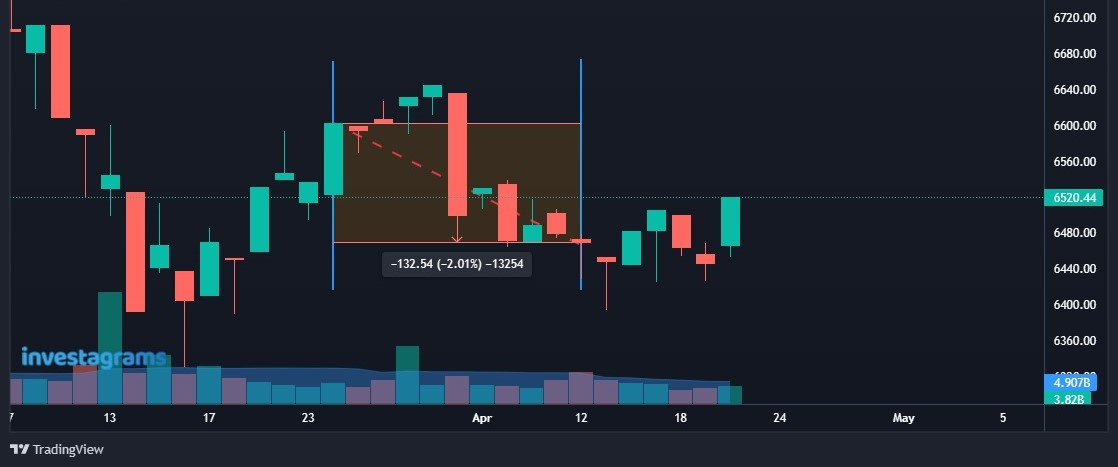
\includegraphics[width=1\textwidth]{./assets/Chapter_4/real_world/actual_PSEI.jpg}
    \caption{PSEI Stock Market Price Trend from March 24 to April 12, 2023}
    \label{fig:psei_actual}
\end{figure}
\FloatBarrier
\textit{Note: The figure above was generated using the chart tool from Investagrams.com}

However, the loss in PSEI may be attributed to the fact that no specific trading 
strategy was followed, but this is still a fair battle between the two systems - 
as the use of the alamSYS was based solely on its recommendations. Whereas, additional 
technical analysis on the stock market may result in higher alamSYS gains.
\\

Figure \ref{fig:daytoday} depicts the day-to-day gains of both systems to further visualize 
the performance of alamSYS's suggestions in comparison to the performance of 
PSEI.
\begin{figure}[ht]
    \centering
    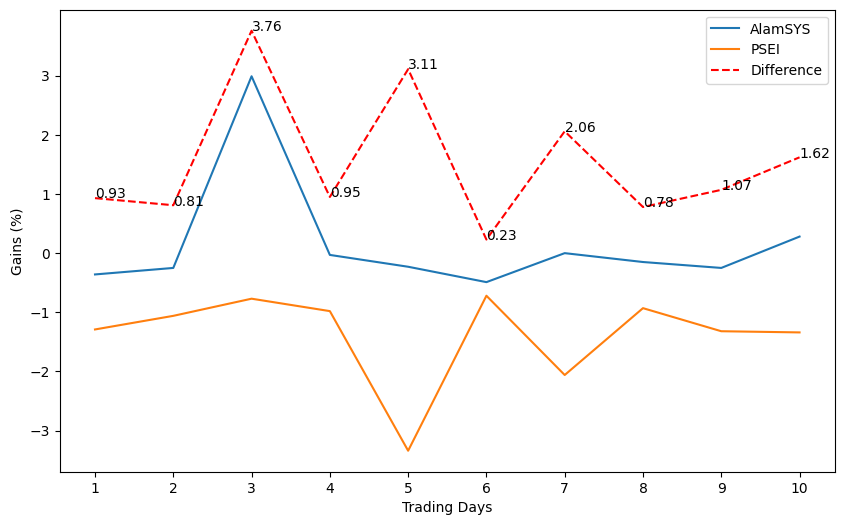
\includegraphics[width=1\textwidth]{./assets/Chapter_4/real_world/comparison.png}
    \caption{Comparison Between the Day-to-day Gains of alamSYS and PSEI}
    \label{fig:daytoday}
\end{figure}
\FloatBarrier

The above figure additionally demonstrates how the alamSYS performs better 
on a daily basis compared to the PSEI, highlighted by the 'Difference' line.  
Whereas the alamSYS performed better than the PSEI by 0.93\%, 0.81\%, 3.76\%, 
0.95\%, 3.11\%, 0.23\%, 2.06\%, 0.78\%, 1.07\%, and 1.62\% over a 10-day 
period. Also, even though the cumulative return was positive, 
the alamSYS's day-to-day performance still yielded negative returns, 
It is worth noting, however, that it was able to reduce the risk of further 
losses, as can be observed in Figure \ref{fig:daytoday}.


